\section{Execution Provenance and Supporting Displays}
\label{app:execution_details}

\subsection{Protocol Amendments and Provenance}

The execution history contains two documented amendments. First, the v1 feasibility run stops before model training on Texas because one class contains a single node and cannot populate the frozen three-way split. Before comparative assembly or evaluation, an outcome-independent eligibility amendment excludes Texas, assigns a new run identifier, and restarts all remaining datasets from zero without changing models, splits, seeds, thresholds, metrics, or inference. Second, after a blinded wall-clock timeout on Squirrel, an execution-only amendment increases the per-dataset limit from 30 to 90 minutes. No comparative outcome is inspected, and all scientific settings remain unchanged. The completed v2 artifacts retain the amendments and exclude the aborted v1 records from analysis.

Here ``prospective'' refers specifically to newly generated records for the pre-specified primary analysis, produced after the specification and scoring implementation were frozen. Legacy aggregate results inspected during exploratory work are not part of this analysis because they lack consistent paired outcomes and decision-time provenance. The public release provides the frozen snapshot, file digests, and mappings to execution provenance, but it does not expose the private predecessor history; the auditable claim is therefore about the released primary run rather than the entire earlier research timeline.

\subsection{Threshold Provenance}

The exact Combined thresholds were not inherited verbatim from an earlier committed rule or derived through a prospective threshold sweep. They first appeared in the frozen specification and scorer after legacy aggregate inspection and before the primary records. Dated source provenance remains in the author archive. The public snapshot documents the released run, while the private predecessor history remains inaccessible.

\subsection{Regret--Coverage Display}
\label{app:coverage_display}

\begin{figure}[t]
\centering
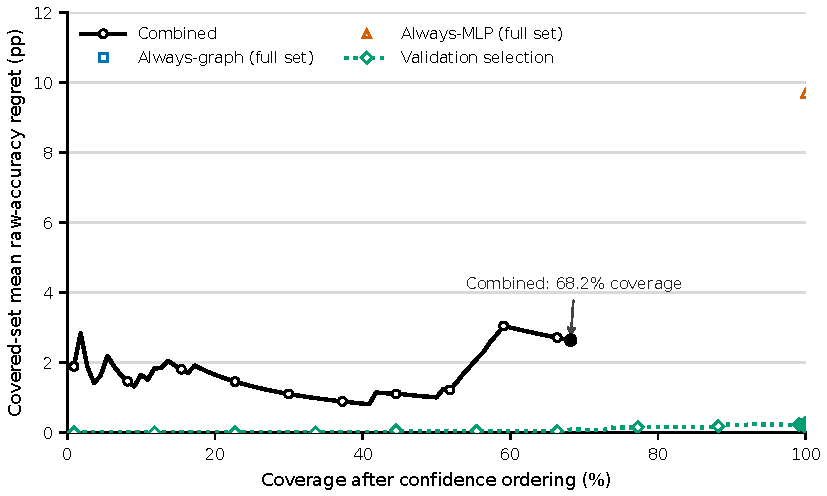
\includegraphics[width=0.82\linewidth]{results/diagnostic/route_a_prospective_v2/analysis/prospective_regret_coverage.pdf}
\caption{Descriptive regret--coverage display from the frozen confidence scores. For Combined and validation selection, coverage increases as lower-confidence eligible decisions enter. Always-graph and always-MLP have constant confidence and therefore appear only as full-set endpoints. The ordinate is covered-set mean raw-accuracy regret, not selection error under the one-point target margin. The Combined curve ends at 68.2\% because 35 units abstain and fallback decisions are not added to this display. The pre-specified primary analysis remains full-set regret with dataset-level inference.}
\label{fig:regret_coverage}
\end{figure}

Figure~\ref{fig:regret_coverage} shows the precomputed descriptive curves for Combined and validation selection, together with the two constant policies at their identifiable full-set endpoints. Raising confidence within the Combined rule does not reveal a sustained regret region comparable to the low-regret reference policies: its final covered-set regret is 2.64 points at 68.2\% coverage, compared with full-set regrets of 0.26 for always-graph and 0.22 for validation selection. This display is a sensitivity summary only and does not replace the predeclared full-set comparison.
